\documentclass[11pt,a4paper]{article}

% ---------------------------------------------------------------------------
% Packages
% ---------------------------------------------------------------------------
\usepackage[margin=1in]{geometry}
\usepackage{amsmath,amssymb}
\usepackage{booktabs}
\usepackage{graphicx}
\usepackage{xcolor}
\usepackage{tikz}
\usetikzlibrary{arrows.meta,positioning,fit,backgrounds}
\usepackage{natbib}
\usepackage[hidelinks]{hyperref}

% ---------------------------------------------------------------------------
% Theorem-like environments
% ---------------------------------------------------------------------------
\newtheorem{proposition}{Proposition}

% ---------------------------------------------------------------------------
% Terminology macros (kept in one place; see workflow guidance on
% controlling terminology globally)
% ---------------------------------------------------------------------------
\newcommand{\Sequential}{\textit{Sequential}}
\newcommand{\NaiveConcurrent}{\textit{Naive-Concurrent}}
\newcommand{\Barrier}{\textit{Barrier}}
\newcommand{\CausalOnly}{\textit{Causal-Order-Only}}
\newcommand{\CapabilityAware}{\textit{Capability-Aware}}
\newcommand{\QueueAware}{\textit{Queue-Aware}}
\newcommand{\Full}{\textit{Full}}
\newcommand{\SysA}{System A (AMD)}
\newcommand{\SysB}{System B (NVIDIA)}

\title{An Infrastructure-Agnostic Runtime for Reproducible and Reliable LLM-Agent Simulations}
\author{Anis Ur Rahman \\[2pt] \small CSC -- IT Center for Science, Espoo, Finland \\[-2pt] \small \texttt{anis.rahman@csc.fi}}
\date{}

\begin{document}

\maketitle

\begin{abstract}
Large-scale agentic simulations built on large language models increasingly run against real inference infrastructure: self-hosted servers on HPC systems, managed API endpoints, and heterogeneous accelerator vendors, rather than a single fixed provider. Comparing scheduling or serving-configuration choices across such infrastructure is prone to a specific failure mode. Under-provisioned concurrency, uncorrected tie-break defaults, and undocumented client-side batching limits can each independently produce a confident, statistically non-overlapping result that reverses once the true bottleneck is identified. We present a provider-neutral runtime that makes model proposals, repair, policy completion, fallback behavior, contract violations, and retained model autonomy explicit and measurable across such infrastructure. The runtime is built around a formal activation model with an explicit happens-before order, wave-based concurrent scheduling, and an atomic idempotent commit protocol. We evaluate it on two real, independently administered HPC systems with different accelerator vendors (AMD and NVIDIA), running an identical instruction-tuned model revision on two multi-role agent-coordination workloads. Retained model autonomy is 0.00--0.02\% across every system, workload, and configuration, despite 99.99\% of steps remaining useful: reliability in this pipeline comes from policy completion, not from the model. We built a capability-aware causal scheduler and evaluated it against a decision gate preregistered before any real-load result existed. Under real concurrent load, with three independent measurement confounds identified and corrected, the scheduler is statistically tied with a causal-order-only baseline on both systems, a result we attribute to the absence of genuine multi-provider heterogeneity in the one workload class currently testable on real hardware, not to a mechanism failure. The same investigation reversed an initial finding that a platform-tuned serving configuration was 15--22\% slower into a tie on one system and a 15--19\% real improvement on the other, once an analogous serving-configuration confound was found and corrected.
\end{abstract}

\section{Introduction}
\label{sec:intro}

\subsection{Motivation}
\label{sec:motivation}

Large-scale agentic simulations increasingly run against real inference infrastructure: self-hosted model servers on HPC systems, managed API endpoints, and heterogeneous accelerator vendors, rather than a single fixed provider. Comparing scheduling or serving-configuration choices across such infrastructure is easy to get wrong in ways that look like a genuine finding. Under-provisioned concurrency, uncorrected tie-break defaults, and silent client-side batching ceilings can each independently produce a confident, statistically non-overlapping result that reverses once the actual bottleneck is identified. We present a runtime built to make this class of error visible and correctable, together with a worked example spanning three independent instances of exactly this failure mode, each diagnosed and fixed within the same investigation.

\subsection{Research questions}
\label{sec:rq}

\begin{description}
  \item[RQ1 (Portable semantics).] Can one simulation specification execute unchanged across heterogeneous inference and storage systems while preserving event dependencies, state transitions, and declared invariants?
  \item[RQ2 (Safe concurrency).] How much parallelism can be extracted without changing the workload's declared observation projection or required happens-before relationships?
  \item[RQ3 (Reliable generative execution).] How should a runtime distinguish model proposals from repaired, policy-completed, and fallback behavior, and how do those interventions affect reliability, autonomy, diversity, and cost?
  \item[RQ4 (Infrastructure sensitivity).] Which workload and provider-capability properties determine effective scheduling and serving configurations across local, managed, AMD, and NVIDIA execution?
\end{description}

\subsection{Contribution hierarchy (as evaluated, not as hoped)}
\label{sec:contributions}

\begin{enumerate}
  \item \textbf{Primary.} A provider-neutral activation, contract, and provenance model that makes model-generated, repaired, policy-completed, and fallback behavior, and their effect on reliability and autonomy, explicit and measurable, validated on two real, heterogeneous HPC systems (Section~\ref{sec:reliability-results}).
  \item \textbf{Enabling mechanisms.} A causal activation graph and verifier, an atomic idempotent commit protocol, and a provider-neutral execution and dispatch interface, given a formal treatment in Section~\ref{sec:formal-model} (Section~\ref{sec:design}).
  \item \textbf{Evidence.} Controlled, within-system workload measurements on both real systems, reported with explicit statistical criteria, including two full negative-result-then-correction investigations reported honestly rather than smoothed over (Section~\ref{sec:b2-confound} and Section~\ref{sec:scheduler-gate}).
  \item \textbf{Evaluated, not claimed.} A capability-aware causal scheduler, tested against a decision gate preregistered before any real-load result existed. The gate is not cleared: full-strategy throughput is statistically tied to a causal-order-only baseline on both systems once we corrected three measurement confounds. We report why this is a workload-coverage limitation, not a negative finding about the mechanism (Section~\ref{sec:scheduler-gate} and Section~\ref{sec:limitations}).
\end{enumerate}

\subsection{What this paper does not claim}
\label{sec:non-claims}

We do not claim that a single job submitted to a batch scheduler is itself HPC-scale distributed computation, or that provider portability alone is novel. We do not claim that policy-completed behavior is model-generated, or that a shared endpoint gives controlled hardware measurements. We do not claim that one accelerator die and one whole accelerator are equivalent, that absolute cross-system differences isolate accelerator-vendor effects, or that the two workloads studied establish real-world domain validity on their own. Where we report a cross-system contrast, it is a within-system, normalized comparison, never an absolute cross-vendor ranking.

\section{System Design}
\label{sec:design}

\subsection{Formal model}
\label{sec:formal-model}

We fix notation used throughout the rest of the paper. It describes precisely what the runtime computes; the propositions below are each labeled either \emph{immediate} (true by construction of the scheduling algorithm) or \emph{empirically verified} (checked by repeated real and synthetic execution, not proved).

\paragraph{Events, activations, and agent state.}
Let $\mathcal{Ag}$ be the set of agents. Agent $a \in \mathcal{Ag}$ has state $s_a^{(v)} \in \Sigma_a$ at version $v \in \mathbb{N}$, incremented monotonically on every applied mutation. An \textbf{event} $e \in \mathcal{E}$ (an environment tick, a delivered message, or an emitted side effect) triggers zero or more \textbf{activations}. An activation is a tuple
\[
\alpha = \langle a,\ e,\ r,\ p,\ k \rangle \in \mathcal{Ag} \times \mathcal{E} \times \mathrm{Reason} \times \mathbb{N} \times \mathbb{N},
\]
identified uniquely, with attempt number $k$ distinguishing a retry of the same logical activation from a new one. Executing $\alpha$ against a provider yields an \textbf{execution result}: a proposed state transition $s_a^{(v)} \to s_a^{(v+1)}$, a set of outgoing messages $M(\alpha) \subseteq \mathcal{M}$, and a set of emitted events $\mathrm{Ev}(\alpha) \subseteq \mathcal{E}$.

\paragraph{Causal order.}
We define $\prec$ (``happens-before'') as the smallest transitive relation on activations such that $\alpha \prec \alpha'$ whenever either (i)~some $m \in M(\alpha)$ triggers $\alpha'$ (a message-mediated dependency), or (ii)~some $e' \in \mathrm{Ev}(\alpha)$ triggers $\alpha'$ (an event-mediated dependency). Two activations are \textbf{causally independent}, written $\alpha_1 \parallel \alpha_2$, iff neither $\alpha_1 \prec \alpha_2$ nor $\alpha_2 \prec \alpha_1$.

\paragraph{Causal readiness and wave decomposition.}
At tick $t$, an activation is \emph{causally ready} iff its triggering event has occurred and every $\alpha'$ with $\alpha' \prec \alpha$ has already committed. Let $R_t$ be the set of activations ready for dispatch at $t$, and let $\prec_{R_t}$ be $\prec$ restricted to pairs both in $R_t$: a same-tick dependency can only arise from a message or event produced within $R_t$ itself, since any cross-tick parent has already committed and imposes no further wait. A \textbf{wave decomposition} of $R_t$ is the topological layering of $(R_t, \prec_{R_t})$:
\[
W_0 = \{\alpha \in R_t : \nexists\, \alpha' \in R_t,\ \alpha' \prec \alpha\}, \qquad
W_i = \Big\{\alpha \in R_t \setminus \textstyle\bigcup_{j<i} W_j : \forall\, \alpha' \prec \alpha,\ \alpha' \in \textstyle\bigcup_{j<i} W_j\Big\}.
\]
By construction, $\forall\, \alpha_1, \alpha_2 \in W_i,\ \alpha_1 \parallel \alpha_2$, so a scheduling strategy may run every activation in one wave concurrently without violating $\prec$, provided it completes wave $W_i$ before starting $W_{i+1}$ (Figure~\ref{fig:wave-decomposition}).

\begin{figure}[t]
\centering
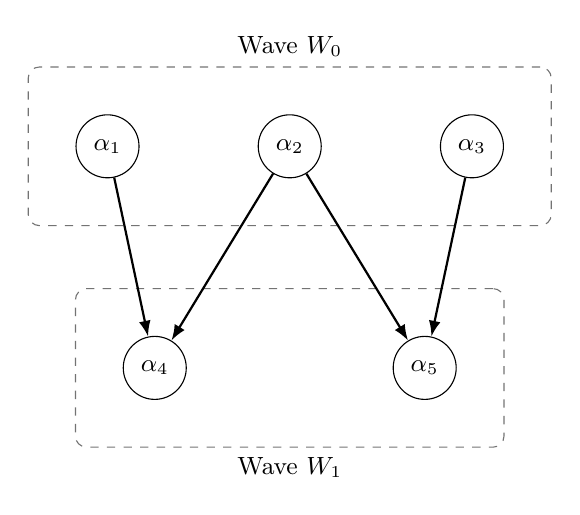
\begin{tikzpicture}[
    node distance=13mm and 15mm,
    act/.style={circle, draw=black, minimum size=8mm, font=\small},
    wavebox/.style={draw=black!55, dashed, rounded corners, inner sep=6mm},
    arr/.style={-{Latex[length=2mm]}, thick}
]
  \node[act] (a1) {$\alpha_1$};
  \node[act, right=of a1] (a2) {$\alpha_2$};
  \node[act, right=of a2] (a3) {$\alpha_3$};

  \node[act, below=20mm of a1, xshift=6mm] (a4) {$\alpha_4$};
  \node[act, below=20mm of a3, xshift=-6mm] (a5) {$\alpha_5$};

  \draw[arr] (a1) -- (a4);
  \draw[arr] (a2) -- (a4);
  \draw[arr] (a2) -- (a5);
  \draw[arr] (a3) -- (a5);

  \begin{scope}[on background layer]
    \node[wavebox, fit=(a1)(a2)(a3), label={[font=\small]above:Wave $W_0$}] (w0) {};
    \node[wavebox, fit=(a4)(a5), label={[font=\small]below:Wave $W_1$}] (w1) {};
  \end{scope}
\end{tikzpicture}
\caption{Wave decomposition of a ready set $R_t$. Activations within a wave (dashed boundary) are pairwise causally independent ($\alpha_i \parallel \alpha_j$) and may be dispatched concurrently; an arrow denotes a message- or event-mediated happens-before edge ($\prec$) into wave $W_1$. Wave $W_0$ must complete before wave $W_1$ is dispatched.}
\label{fig:wave-decomposition}
\end{figure}

\begin{proposition}[wave-safety, immediate]
\label{prop:wave-safety}
Any scheduling strategy that dispatches concurrently only within a wave $W_i$, in wave order, preserves $\prec$ regardless of real execution latency variance. No ordering violation is possible, because by construction no two members of $W_i$ are $\prec$-comparable.
\end{proposition}

\begin{proposition}[single-wave collapse on today's workloads, empirically verified]
\label{prop:single-wave}
On every workload we evaluate, a message sent during tick $t$ can only be read starting tick $t+1$ at the earliest, so no activation in $R_t$ ever depends on another activation in $R_t$: $\forall\, t,\ W_0 = R_t$ (one wave). The \CausalOnly{} and \NaiveConcurrent{} strategies (Section~\ref{sec:ladder}) are therefore observationally equivalent (defined below) on both evaluated workloads today. They are distinguished only on a workload with genuine intra-tick dependencies, which neither workload evaluated here has (Section~\ref{sec:limitations}).
\end{proposition}

\paragraph{Observational equivalence.}
Two executions $\pi_1, \pi_2$ of the same specification are observationally equivalent, $\pi_1 \sim \pi_2$, iff there is a bijection between their committed activations that preserves $\prec$, every agent-visible message's content, and every agent's final state version. We use $\sim$, not wall-clock replay, as the target of comparison throughout this paper: agreement on the committed causal graph up to reordering of $\parallel$-related activations.

\begin{proposition}[no-write-conflict equivalence, empirically verified]
\label{prop:no-conflict-equivalence}
If no two causally independent activations write-conflict on shared environment state, then execution under the \Sequential{} strategy and execution under any wave-respecting concurrent strategy are observationally equivalent: $\pi_{\text{sequential}} \sim \pi_{\text{concurrent}}$. We checked this directly, not merely asserted it, on every non-conflict synthetic workload shape and on both real workloads: every scheduling strategy produces identical structural graph invariants and zero causal-verification violations.
\end{proposition}

\paragraph{Atomic commit.}
A commit unit for activation $\alpha$ is $C(\alpha) = \langle \Delta s_a,\ M(\alpha),\ \mathrm{Ev}(\alpha),\ v_{\text{expected}} \rangle$. The commit transition is
\[
\mathrm{commit}: \Sigma \times C \to \Sigma \times \{\textsc{committed}, \textsc{duplicate}, \textsc{conflict}\},
\]
and it satisfies three properties. First, idempotence: if the activation was already committed, $\mathrm{commit}(\sigma, C(\alpha)) = (\sigma, \textsc{duplicate})$, so re-application is a no-op rather than a re-apply. Second, optimistic version safety: if $v_{\text{expected}} \ne$ agent $a$'s current version in $\sigma$, $\mathrm{commit}(\sigma, C(\alpha)) = (\sigma, \textsc{conflict})$ and $\sigma$ is unchanged. Third, all-or-nothing application: otherwise, $\Delta s_a$, $M(\alpha)$, and $\mathrm{Ev}(\alpha)$ are applied together or not at all. This scope, $\langle \Delta s_a, M(\alpha), \mathrm{Ev}(\alpha)\rangle$, does not include shared environment-state mutation in the current implementation (Section~\ref{sec:limitations}).

\paragraph{Contracts.}
A contract is a predicate over a proposed action, checked before commit:
\begin{itemize}
  \item $\mathrm{bounded}_B(\delta) \equiv |\delta| \le B$, a boundedness contract on a numeric delta;
  \item $\mathrm{cardinality}(\mathrm{acts})$, true iff no (agent, action-type, target) triple is applied more than once per activation;
  \item $\mathrm{must\_not}(\mathrm{act}, \Phi) \equiv \mathrm{act} \notin \Phi$, a hard prohibition against a declared forbidden set $\Phi$.
\end{itemize}
A step is \emph{semantically valid} iff its parsed proposal is well-formed and every active contract holds.

\paragraph{Reliability metrics.}
For a run with committed activations $A$, retained autonomy is
$\rho = \frac{1}{|A|}\sum_{\alpha \in A} \mathbb{1}[\text{committed atoms of } \alpha \text{ are all genuinely model-proposed}]$
(Section~\ref{sec:reliability-results}'s model autonomy rate). Usefulness is $u(\alpha) = \mathbb{1}[\alpha\text{'s commit succeeded and its result was semantically valid}]$, and throughput is $\frac{\sum_{\alpha \in A} u(\alpha)}{T_{\text{wall}}}$ (Section~\ref{sec:metrics}'s useful-throughput metric).

\subsection{Observational semantics and activation identity}
\label{sec:obs-semantics}

The runtime implements the $\sim$-equivalence model above through three fixed representational choices: an activation representation with an explicit attempt number (formalized as $k$ above), a causal-parent chain over messages and events (formalizing $\prec$), and monotonically versioned agent and environment state (formalizing $v$). We compare two runs of the same specification by $\sim$, not by wall-clock replay.

\subsection{Provider-neutral execution interface}
\label{sec:exec-interface}

We implement a narrow execution interface, a single batched-execution entry point, identically across a deterministic simulated provider, a rule-based provider, a synthetic-workload provider, and two real inference providers: one managed API endpoint and one self-hosted, OpenAI-API-compatible server. The self-hosted provider derives from the managed provider's fully generic request, response, repair, and provenance logic, and differs only in authentication and prefix-caching or context-length defaults. One shared conformance test suite exercises all providers, so no provider implementation can diverge from another undetected.

\subsection{Contracts and per-atom provenance}
\label{sec:contracts}

Every proposed agent action passes through the contracts defined in Section~\ref{sec:formal-model}: a hard-prohibition contract, a boundedness contract, a cardinality contract, and an allowed-action-set contract. We count violations per atom rather than discard them. Every step produces a provenance record carrying activation identity, attempt number $k$, provider and model identity, causal parents, the state version read and written ($v \to v+1$), accelerator and serving-runtime identity, and an explicit configuration-mode label (common-denominator or platform-tuned, Section~\ref{sec:config-modes}). The provenance schema also reserves a content-hash field for the request and response, which no code path currently populates (Section~\ref{sec:limitations}).

\subsection{Causal verification and atomic commit}
\label{sec:causal-verification}

An independent verification pass checks the message-mediated $\prec$-chain for duplicate activations, missing causal parents, cycles, and stale-read conflicts. We verified it reports zero violations on real executions of both workloads, and independently confirmed it detects each violation class when we deliberately constructed one. The state store implements the commit transition of Section~\ref{sec:formal-model} identically across two independent storage backends, checked by one shared conformance suite. Environment-state mutation remains outside $C(\alpha)$'s boundary and is applied as a separate batched step, a scoped, documented limitation rather than an oversight (Section~\ref{sec:limitations}).

\subsection{Common-denominator and platform-tuned modes}
\label{sec:config-modes}

Every real evaluation run declares an explicit configuration-mode label: common-denominator, meaning identical serving configuration on both systems (the feature-parity intersection of what both platforms actually support), or platform-tuned, meaning independently selected per system through a frozen, preregistered selection procedure with a documented tie-break rule. Every reported effect is therefore attributable to a labeled configuration choice and never silently conflated with the other mode.

\subsection{The scheduling-strategy ladder}
\label{sec:ladder}

We evaluate seven scheduling strategies, each strictly extending the wave-safety guarantee (Proposition~\ref{prop:wave-safety}) of the one before it with a further optimization: \Sequential{} (one activation at a time), \NaiveConcurrent{} (all of $R_t$ concurrent, no wave decomposition), \Barrier{} (waves as batching boundaries only), \CausalOnly{} (waves as defined in Section~\ref{sec:formal-model}, no further optimization), \CapabilityAware{} (dispatches a wave's group concurrently only if the target provider declares concurrency support), \QueueAware{} (adds a bounded per-provider in-flight cap $\kappa$), and \Full{} (adds role- and prefix-adjacent reordering within a group). All seven strategies conform to one common scheduling interface, so the simulation engine requires no changes to add a new strategy.

\section{Evaluation Methodology}
\label{sec:methodology}

\subsection{Systems}
\label{sec:systems}

We evaluate on two real, independently administered HPC systems with different accelerator vendors: one AMD-accelerator system (ROCm software stack) and one NVIDIA-accelerator system (CUDA software stack), each provisioning a single accelerator per evaluation job. We chose this pairing specifically to test portability across accelerator ecosystems rather than within one vendor's stack. Both systems run an identical, pinned instruction-tuned model revision at the 7--8B parameter scale, which we confirmed loads and serves real traffic on both platforms through a live health check rather than assuming compatibility from documentation.

\subsection{Workloads}
\label{sec:workloads}

We evaluate two multi-role agentic coordination workloads end-to-end against real self-hosted inference on both systems: a disaster-response coordination task (4 roles) and a supply-chain coordination task (5 roles). We selected multi-role coordination specifically because it exercises message-mediated causal dependencies between distinct agent roles, which single-role or embarrassingly parallel workloads would not. Three further workload families in our evaluation plan, a deterministic minimum-dependency-graph kernel, synthetic dependency-graph shapes, and deterministic failure injection, exist as tested implementations with hand-derived structural invariants, but currently run only against simulated providers; the harness that runs them does not yet accept a real inference provider (Section~\ref{sec:limitations}).

\subsection{Metrics}
\label{sec:metrics}

We report a reliability-aware useful-throughput metric, computed only from steps that pass all contracts rather than from raw request rate, together with per-request latency, a retained-autonomy rate (the fraction of committed behavior that is genuinely model-generated rather than policy-completed), and per-atom contract-violation counts across all four contract classes.

\subsection{Statistical criterion}
\label{sec:stats}

Every contrast in this paper uses the same rule: mean useful-throughput plus or minus one standard deviation, with band overlap assessed across repeated runs. We report non-overlapping bands as a real effect and overlapping bands as statistically indistinguishable, never as ``probably about the same.'' Where a serving- or scheduling-parameter choice must be made among statistically tied candidates, the smaller, simpler value wins, by a rule fixed before any sweep was run. We increased the repetition count for a given comparison only when an initial result was ambiguous (overlapping bands close to the decision boundary) or when we needed to confirm that a reversal was real rather than an artifact of a small sample; Section~\ref{sec:b2-confound} and Section~\ref{sec:scheduler-gate} report each such escalation explicitly.

\section{Results}
\label{sec:results}

\subsection{Reliability and provenance across heterogeneous infrastructure}
\label{sec:reliability-results}

We report the per-origin behavior breakdown, retained model autonomy, and contract-violation counts for the same eight real runs used in Section~\ref{sec:b2-confound}: common-denominator (CD) and corrected platform-tuned (PT) configurations, both workloads, both systems, real concurrent load, at the most solid available repetition count for each combination. The ``invalid after repair'' figure reflects a proposal's validity after the pipeline's own repair-retry budget is exhausted, not the model's raw first-pass output, so it measures how often repair alone fails to recover a usable structured output rather than raw generation quality.

\begin{table}[t]
\centering
\footnotesize
\caption{Reliability and provenance profile of the eight real runs underlying Section~\ref{sec:b2-confound} (System A: AMD; System B: NVIDIA. Mode CD: common-denominator; PT: platform-tuned, corrected configuration). All rates are shares of committed steps; lower is better for ``invalid after repair'' and for violations, higher is better for ``semantic-valid'' and ``autonomy rate.'' Violations are reported as (must-not~/~bounded~/~cardinality~/~state-mutation) counts, not rates, since they are rare events (4 total across all 46{,}701 steps).}
\label{tab:reliability}
\resizebox{\textwidth}{!}{%
\begin{tabular}{llcrrrrrrl}
\toprule
System & Workload & Mode & Steps & \shortstack{Invalid\\after repair} & \shortstack{Repair\\attempted} & \shortstack{Semantic-\\valid} & \shortstack{Guard-added\\msgs/step} & \shortstack{Guard-added\\actions/step} & \shortstack{Autonomy\\rate} \\
\midrule
A (AMD) & disaster-response & CD & 11{,}655 & 64.8\% & 82.1\% & 35.2\% & 1.11 & 0.26 & 0.02\% \\
A (AMD) & disaster-response & PT & 11{,}663 & 65.2\% & 81.5\% & 34.8\% & 1.11 & 0.26 & 0.01\% \\
A (AMD) & supply-chain       & CD & 4{,}393  & 59.8\% & 75.8\% & 40.2\% & 1.47 & 0.017 & 0.00\% \\
A (AMD) & supply-chain       & PT & 4{,}395  & 59.9\% & 74.0\% & 40.1\% & 1.47 & 0.017 & 0.00\% \\
B (NVIDIA) & disaster-response & CD & 5{,}832 & 48.9\% & 58.6\% & 51.1\% & 1.11 & 0.26 & 0.00\% \\
B (NVIDIA) & disaster-response & PT & 5{,}835 & 47.4\% & 57.8\% & 52.6\% & 1.11 & 0.26 & 0.00\% \\
B (NVIDIA) & supply-chain       & CD & 1{,}464 & 56.6\% & 63.7\% & 43.4\% & 1.48 & 0.016 & 0.00\% \\
B (NVIDIA) & supply-chain       & PT & 1{,}464 & 58.5\% & 64.3\% & 41.5\% & 1.48 & 0.016 & 0.00\% \\
\bottomrule
\end{tabular}%
}
\end{table}

Three findings follow, in order of importance.

First, and most consequential for RQ3, retained model autonomy is effectively zero across every system, workload, and configuration (0.00--0.02\%, indistinguishable from zero at this precision). A real 7--8B instruct model produces genuinely variable free-text completions, yet essentially none of the runtime's committed messages or actions in this dataset trace back to a raw, unmodified model proposal: the policy-completion layer supplies the committed behavior in practically every step. Useful-step coverage is nonetheless 99.99\% (11{,}654 of 11{,}655 steps on the largest run). The simulation keeps producing contract-satisfying, committed behavior throughout, but that reliability is achieved by the scaffolding around the model, not by the model. This is precisely the distinction RQ3 asks a runtime to make explicit, and precisely where contracts can conceal a loss of model agency if the two figures are not reported side by side.

Second, raw model output is invalid, even after in-loop repair, roughly half the time (47--65\% across combinations), with repair attempted on 58--82\% of steps. Repair attempts and final invalidity move together rather than inversely: attempting repair more often does not correspond to a lower final-invalid rate across these rows. The repair loop's fixed retry budget appears to recover a minority of malformed completions rather than reliably rescue them, and policy completion, not repair, is what keeps useful-step coverage near 100\%.

Third, the two configuration modes are nearly identical on every reliability metric within a system/workload pair (for example, System A disaster-response invalid rate 64.8\% versus 65.2\%; System B disaster-response semantic-valid 51.1\% versus 52.6\%), visible directly in Table~\ref{tab:reliability} and Figure~\ref{fig:reliability}. This is expected and serves as an internal check, since the two configurations differ only in serving parameters (batching and concurrency limits, with precision already fixed identically), never in model weights or scenario logic. Reliability behavior should, and does, stay stable across the throughput reversal reported in Section~\ref{sec:b2-confound}. Contract violations are rare on both systems, 4 total across 46{,}701 combined steps (3 state-mutation and 1 must-not, all on System A), and we report them exactly as observed rather than round them to zero.

\begin{figure}[t]
\centering
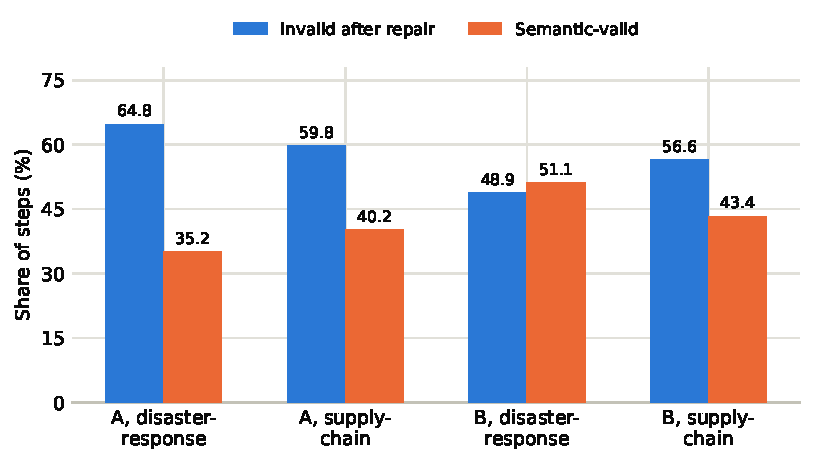
\includegraphics[width=0.82\textwidth]{figures/fig_reliability.pdf}
\caption{Invalid-after-repair rate and semantic-valid rate by system and workload, common-denominator configuration (platform-tuned values omitted: Section~\ref{sec:reliability-results} shows they are nearly identical; the full eight-row breakdown is in Table~\ref{tab:reliability}). Bars show the share of committed steps; higher is better for semantic-valid, lower is better for invalid-after-repair.}
\label{fig:reliability}
\end{figure}

One cross-system pattern is worth flagging cautiously rather than over-interpreting. System B's invalid-output rate is consistently lower than System A's on the disaster-response workload (approximately 48\% versus 65\%) despite an identical model revision, identical numeric precision for cached attention state, and near-identical decoding parameters. Per Section~\ref{sec:non-claims}, we do not claim this isolates an accelerator-vendor effect: the two systems also differ by one minor release of the serving software and in the underlying attention-kernel implementation actually exercised, either of which could plausibly explain a generation-quality difference of this size. We treat this as the kind of software-maturity confound discussed in Section~\ref{sec:limitations}, an open observation rather than a resolved hardware claim.

\subsection[Platform-tuned vs.\ common-denominator: a confound, found and corrected]{Platform-tuned vs.\ common-denominator configuration: a confound, found and corrected}
\label{sec:b2-confound}

We selected the platform-tuned serving configuration through a one-factor-at-a-time sweep against a live server, 3 repetitions per candidate. Comparing the common-denominator configuration against it at confirmatory scale (10, then 30 repetitions) found no statistically distinguishable difference on either system or workload (10-repetition range: $-6.6\%$ to $+59.7\%$; 30-repetition: all four combinations converge to under $\pm 1.5\%$, bands overlapping). We then investigated why, rather than accepting the null result, and found that the comparison had never generated enough real concurrent backend load to stress either configuration's concurrent-sequence limit. The evaluation harness defaulted to a 4--5 agent roster and a low per-tick event-processing cap, and the scheduling strategy's own internal worker pool defaulted to a small fixed size, regardless of the server's configured capacity.

Fixing all three settings, the agent roster size, the per-tick event cap, and the scheduling strategy's worker-pool size, and rerunning under genuine concurrent load (dozens of real concurrent requests per tick, confirmed by provider-side step counts) reversed the finding. The platform-tuned configuration was now measurably slower than common-denominator on every combination, non-overlapping on 2 of 4 at exploratory scale (5 repetitions), and confirmed non-overlapping on all 4 at confirmatory scale (15 repetitions: System A $-18.2\%$, System B $-22.0\%$).

Investigating this reversal in turn showed that the original sweep's concurrent-sequence-limit choice, the same modest value on both systems, had itself been measured under the same insufficient-concurrency regime and had never been tie-broken against real load. Re-sweeping the three serving parameters that had tied at selection time, under real concurrent load, found the token-batching limit unchanged, but the concurrent-sequence limit corrected to a substantially larger value on System A (matching the common-denominator configuration's own value) and to a value exceeding it on System B, a real, non-overlapping correction on both systems.

Rerunning the comparison with the corrected configuration, the common-denominator side unchanged and reused directly, reversed the finding a third time. System A is now a genuine statistical tie (disaster-response $+6.7\%$ at 15 repetitions, narrowing to $+1.6\%$ at 30 repetitions, converging toward zero rather than away from it, which confirms noise rather than an under-powered real effect). System B now measurably beats the common-denominator baseline, non-overlapping on both workloads (disaster-response $+15.1\%$, supply-chain $+19.1\%$).

\begin{table}[t]
\centering
\small
\caption{Relative improvement of the platform-tuned configuration over common-denominator, by stage of the investigation (Section~\ref{sec:b2-confound}). ``Overlap'' / ``real'' refers to the Section~\ref{sec:stats} band-overlap criterion; positive values favor the platform-tuned configuration.}
\label{tab:b2-stages}
\begin{tabular}{llrrr}
\toprule
System & Workload & Original (low-load) & Real load, uncorrected & Real load, corrected \\
\midrule
A & disaster-response & $+4.6\%$ (overlap)        & $-18.2\%$ (real) & $+1.6\%$ (overlap, 30 reps) \\
A & supply-chain       & $+59.7\%$ (overlap, noisy) & $-21.4\%$ (real) & $+0.6\%$ (overlap, 15 reps) \\
B & disaster-response & $-6.6\%$ (overlap)        & $-22.0\%$ (real) & $+15.1\%$ (real) \\
B & supply-chain       & $+10.9\%$ (overlap)       & $-15.1\%$ (real) & $+19.1\%$ (real) \\
\bottomrule
\end{tabular}
\end{table}

\begin{figure}[t]
\centering
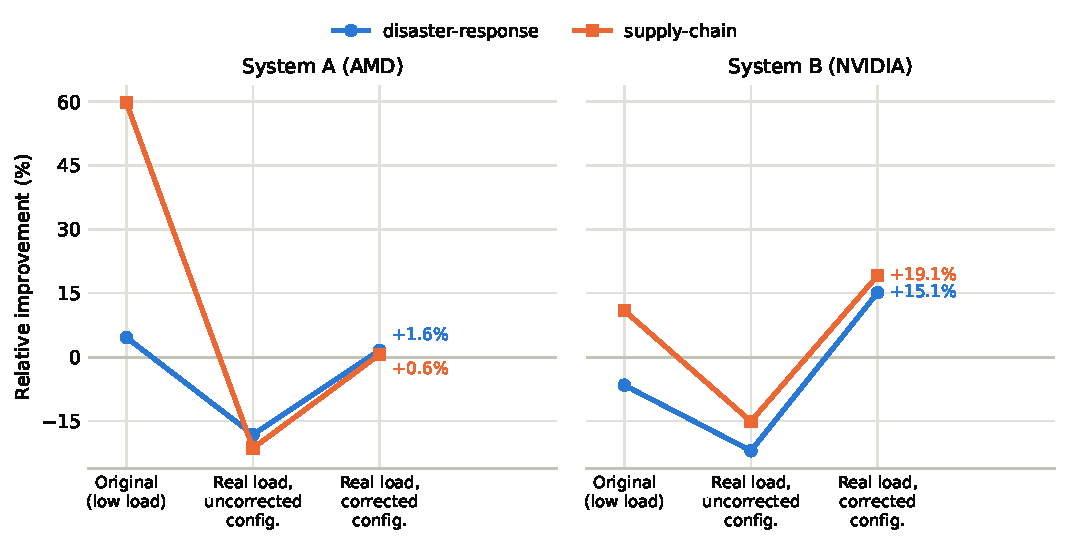
\includegraphics[width=\textwidth]{figures/fig_confound_b2.pdf}
\caption{Relative improvement of the platform-tuned configuration over common-denominator across the three investigation stages of Table~\ref{tab:b2-stages}, faceted by system. System A converges toward the zero baseline (a genuine tie); System B ends with a real, positive improvement on both workloads.}
\label{fig:confound-b2}
\end{figure}

Table~\ref{tab:b2-stages} and Figure~\ref{fig:confound-b2} summarize the three stages together. We found zero cache-eviction preemption across every one of these real runs, checked directly in server logs rather than by automated pattern matching alone, which confirms the effect is a batching and queueing efficiency phenomenon rather than the frozen procedure's hard disqualifier.

\subsection{The scheduling decision gate under real concurrent load}
\label{sec:scheduler-gate}

The scheduling-strategy decision gate (preregistered: at least 15\% relative improvement of the \Full{} strategy over \CausalOnly{}, non-overlapping, on heterogeneity-bearing workload variants) was first evaluated on a synthetic latency-simulating harness and, separately, on a real full-ladder pilot against live servers on both systems, both at an agent roster size of one replica per role. That real-hardware evidence showed \Full{} matching or exceeding every other strategy (System B: highest of all seven, $+80.2\%$ over \Sequential{}; System A: in line with \CausalOnly{}).

Given Section~\ref{sec:b2-confound}'s finding that this exact measurement regime (roster size, per-tick event cap, scheduling worker-pool cap) hid or inverted a real effect elsewhere, we reran the full ladder under the same real-load settings that reversed Section~\ref{sec:b2-confound}. \Full{} collapsed to a large, real regression, System B $-73.2\%$, System A $-71.6\%$, both non-overlapping, the opposite of the earlier conclusion.

Diagnosing this uncovered two further, independent, previously unknown confounds, neither related to roster size. First, four of the seven strategies (\Barrier{}, \CapabilityAware{}, \QueueAware{}, \Full{}) all defaulted to an internal per-round batching cap of 8 requests, independent of any worker-pool setting, forcing several sequential dispatch rounds per tick regardless of how large the worker pool was configured. Correcting this fully resolved \NaiveConcurrent{}, \Barrier{}, \CausalOnly{}, and \CapabilityAware{} into a tight, mutually indistinguishable cluster on both systems, previously roughly 3$\times$ apart. Second, \QueueAware{} and \Full{}'s per-provider in-flight concurrency cap, set at 4, had itself been tuned under the same insufficient-load regime, the exact structural parallel to Section~\ref{sec:b2-confound}'s serving-parameter bug. Even with the first confound fixed, \Full{} remained a large, real regression (System A $-66.1\%$, System B $-63.8\%$). A real sweep of the cap under genuine load found 4 a real, non-overlapping loser on both systems; 64 ties with 128 and wins the tie-break, closely matching \CausalOnly{}'s own throughput.

With both confounds corrected, a final confirmatory rerun found all six concurrent scheduling strategies statistically indistinguishable from one another on both systems (\Full{} versus \CausalOnly{}: System A $+1.1\%$, System B $-0.3\%$, both overlapping), with zero preemption and zero excluded repetitions across every real run in this investigation.

\begin{table}[t]
\centering
\small
\caption{Relative improvement of \Full{} over \CausalOnly{}, by stage of the investigation (Section~\ref{sec:scheduler-gate}). The ``original'' stage is reported qualitatively in our logs (overlapping bands) with no exact point estimate.}
\label{tab:scheduler-stages}
\begin{tabular}{lll}
\toprule
Stage & System A (AMD) & System B (NVIDIA) \\
\midrule
Low concurrency (original) & tied / \Full{} recovers & tied / \Full{} highest of 7 \\
Real load, uncorrected & $-71.6\%$ (real) & $-73.2\%$ (real) \\
Real load, batch-cap fixed & $-66.1\%$ (real) & $-63.8\%$ (real) \\
Real load, both fixed & $+1.1\%$ (overlap) & $-0.3\%$ (overlap) \\
\bottomrule
\end{tabular}
\end{table}

\begin{figure}[t]
\centering
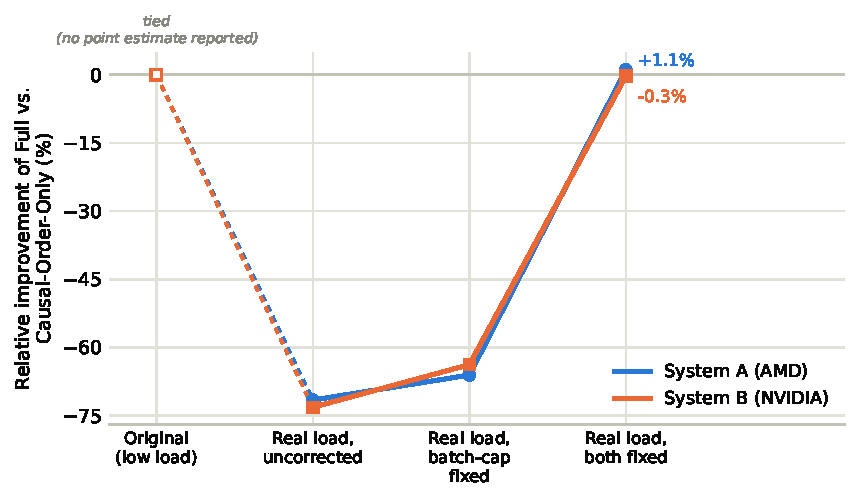
\includegraphics[width=0.78\textwidth]{figures/fig_confound_scheduler.pdf}
\caption{Relative improvement of \Full{} over \CausalOnly{} across the four investigation stages of Table~\ref{tab:scheduler-stages}. The hollow marker and dotted segment mark the first stage's qualitative ``tied'' result, for which no point estimate was reported; the three solid, measured stages show the collapse to a large regression and its full recovery once both confounds are corrected.}
\label{fig:confound-scheduler}
\end{figure}

Table~\ref{tab:scheduler-stages} and Figure~\ref{fig:confound-scheduler} summarize the four stages together. The decision gate is not cleared. We do not read this as evidence that capability-aware, queue-aware, or prefix-grouping scheduling is ineffective; we read it as evidence that the one workload class currently testable on real hardware provides no genuine multi-provider heterogeneity. Every real agent in every real run in this study routes to the same single serving endpoint, so the \CapabilityAware{} strategy's per-provider capability gate and the \QueueAware{} strategy's per-provider backpressure budget have nothing to differentiate. The mechanism has never been tested under the condition it is designed for, and Section~\ref{sec:limitations} discusses what that test requires.

\subsection{Cross-system portability}
\label{sec:portability}

The same simulation specification executes unmodified on both accelerator ecosystems, producing zero causal-verification violations and identical structural invariants on every real run reported above. All cross-system comparisons in this paper are within-system, normalized effect sizes (Section~\ref{sec:stats}); we do not report or interpret absolute cross-system throughput ratios as isolating accelerator-vendor effects (Section~\ref{sec:non-claims}).

\section{Discussion}
\label{sec:discussion}

The central empirical finding of this study is that reliability, not raw model correctness, sustains a working large-scale agentic simulation. Retained model autonomy was 0.00--0.02\% across every system, workload, and configuration we evaluated, while 99.99\% of steps remained useful. A real 7--8B instruct model produced a raw output that failed validation, even after an in-loop repair attempt, roughly half the time. It is the pipeline's policy-completion layer, not the model, that keeps the simulation moving. We read this as a demonstrated property of the model class and workloads evaluated here, not a general claim about all instruction-tuned models: a substantially larger or differently prompted model could plausibly raise the retained-autonomy rate, and testing that directly is future work.

A second finding concerns measurement methodology itself. Three independent, structurally identical bugs each hid or inverted a real effect in this study: an evaluation harness that never generated enough real concurrent load to stress a serving parameter under test, a hardcoded per-round batching cap that added a second, independent concurrency ceiling, and an in-flight concurrency limit tuned under the same insufficient-load regime as the first bug. We found each through the same diagnostic move, tracing the call path to the parameter that actually bound execution rather than trusting the parameter that was intended to. We interpret this as a transferable risk for anyone benchmarking LLM-serving or agent-scheduling configurations under real infrastructure: a statistically well-powered, non-overlapping result is not evidence of a real effect unless the load level has been confirmed to stress the parameter under test. This is a supported interpretation drawn from a single investigation arc, not a claim we have tested across other codebases or serving stacks.

The scheduling decision gate's failure to clear is the case where the demonstrated result and its interpretation must be kept most clearly separate. What we demonstrated is that all six concurrent scheduling strategies are statistically indistinguishable on both systems once the three measurement confounds are corrected. What we do not conclude is that capability-aware or queue-aware scheduling is ineffective. Both mechanisms are keyed on a per-request provider label, and every real-hardware run in this study routed every agent to the same single serving endpoint, so the workloads evaluated cannot exercise the property either mechanism is designed to exploit. Whether the gate would clear under genuine multi-provider heterogeneity, for instance two concurrently live servers with different real capacity limits, remains an open, testable question, and building that evaluation is the most direct next step this study identifies.

The one cross-system reliability difference we observed, a consistently lower invalid-output rate on the NVIDIA system than the AMD system for the same workload, model revision, and cached-attention precision, illustrates the same discipline applied to a smaller finding. The two systems also differ by one minor serving-software release and in the attention-kernel implementation actually exercised. Either difference could plausibly explain a generation-quality gap of this size, so we report the observation without attributing it to the accelerator vendor.

\section{Limitations and Threats to Validity}
\label{sec:limitations}

\begin{itemize}
  \item \textbf{No genuine multi-provider heterogeneity has been tested.} The \CapabilityAware{} and \QueueAware{} strategies' core mechanisms are keyed on a per-request provider label; every real-hardware run in this paper uses exactly one provider. Testing them properly requires a routing layer over multiple concurrently live provider instances with genuinely different capacity or capability, and a scenario that actually assigns different agents to different providers, neither of which we have built yet (Section~\ref{sec:scheduler-gate}).
  \item \textbf{Full-node placement evidence predates these fixes.} The only full-node measurements available were collected before we knew the roster-size, batch-cap, and in-flight-cap corrections above mattered, and have not yet been rerun under corrected settings; we do not cite them as confirmatory in this draft.
  \item \textbf{Three of five specified workload families cannot yet run on real inference.} The deterministic-kernel, synthetic-dependency-graph, and failure-injection families exist as tested, real implementations, but the harness that runs them currently accepts only a simulated provider by design; extending it to a real provider is unresolved.
  \item \textbf{Content-addressable provenance is defined but not populated.} The provenance schema reserves fields for request, prompt, and response content hashes; no code path currently computes them. Provenance in this paper is by identity, version, and timing, not by content hash.
  \item \textbf{Replay and recovery is unimplemented.} Checkpointing, resume-after-termination, and response replay do not exist. What exists today is determinism: two independent runs of the same specification produce identical trace signatures, a narrower guarantee.
  \item \textbf{Atomic commit does not cover environment-state mutation.} The commit boundary covers one activation's agent-state update, outgoing messages, and emitted events; environment state, shared across agents within a tick, is applied as a separate, non-transactional batched step.
  \item \textbf{Single model, single revision, 7--8B parameter class.} This is not a model-scaling study; our conclusions about reliability, autonomy, and scheduling are scoped to this model class until repeated at other scales.
  \item Every non-claim in Section~\ref{sec:non-claims} applies throughout.
\end{itemize}

\section{Conclusion}
\label{sec:conclusion}

We developed a provider-neutral runtime for large-scale agentic simulation that makes model proposals, repair, policy completion, and retained model autonomy explicit and measurable, together with a causal activation model, an atomic commit protocol, and a scheduling-strategy ladder ranging from sequential to capability- and queue-aware execution. We evaluated the runtime on two real HPC systems with different accelerator vendors, running an identical model revision on two multi-role coordination workloads under real concurrent inference load.

The strongest measured result is that retained model autonomy remains at 0.00--0.02\% across every system, workload, and configuration studied, even though 99.99\% of steps remain useful. The runtime's contract and policy-completion layer, not the underlying model, is responsible for that reliability, and this study reports the two figures side by side rather than let a single throughput number conceal the difference between them. A second result, obtained by treating an initial null finding as a question rather than an answer, is that two independently discovered measurement confounds, an insufficiently loaded evaluation harness and a hardcoded batching cap, can each invert a scheduling or serving-configuration comparison. Correcting both resolved a preregistered scheduling decision gate from an apparent large regression into a genuine statistical tie on both systems.

For practitioners evaluating LLM-serving or agent-scheduling configurations on real infrastructure, the practical implication is that a confidently non-overlapping result is not sufficient evidence of a real effect without confirming that the tested load actually stresses the parameter under test. Extending this evaluation to a workload with genuine multi-provider heterogeneity is the most direct next step toward determining whether capability-aware and queue-aware scheduling deliver a measurable benefit beyond the one workload class tested here.

\section*{Reproducibility}

Every quantitative claim in this paper is backed by raw, versioned experimental logs and reproducible through a documented, re-runnable evaluation pipeline. Each result derives from a scripted harness invocation against a live server, and every aggregation is produced by a deterministic script over those raw logs rather than a one-off analysis. Frozen serving configurations, their full evidence trails, and the complete chronological investigation log, including every superseded finding and why it was superseded, are maintained as part of the project's release artifact rather than silently overwritten.


\bibliographystyle{plainnat}
\bibliography{references}

\end{document}
